\documentclass[11pt]{article}

\usepackage{setspace}
\usepackage{amsmath}
\usepackage{enumitem}
\usepackage{amsfonts} 
\usepackage{mathtools}
\usepackage{relsize}
\usepackage{graphicx}
\usepackage[top=2cm,bottom=2cm,left=2.5cm,right=2.5cm,marginparwidth=1.75cm]{geometry}
\setlength{\parindent}{0cm}
\usepackage{listings}
\usepackage{clrscode3e}
\usepackage{graphicx}
\def \n {\par \vspace{\baselineskip}}

\def\lc{\left\lceil}   
\def\rc{\right\rceil}
\def\lf{\left\lfloor}   
\def\rf{\right\rfloor}

\title{\vspace{-1.0cm}PHYS 2303 Homework 3}
\author{Fletcher Gornick}
\date{February 6, 2022}

\spacing{1.5}
\begin{document}
 \maketitle 
 \section*{Chapter 3 Problem 93}
 An insulated vessel contains 1.5 moles of helium at 2 atm. The gas initially occupies a 
 volume of 5 L. As a result of the adiabatic expansion the pressure of the gas is reduced 
 to 1 atm. \\

 (a) Find the volume and temperature of the final state. \\

 (b) Find the temperature of the gas in the initial state. \\

 (c) Find the work done by the gas in the process. \\

 (d) Find the change in the internal energy of the gas in the process. \\
 \newpage

 \section*{Chapter 4 Problem 35}
 A Carnot engine operates between reservoirs at 600 and 300 K. If the engine absorbs 100 J 
 per cycle at the hot reservoir, what is its work output per cycle?
 \newpage

 \section*{Chapter 4 Problem 50}
 One mole of an ideal gas doubles its volume in a reversible isothermal expansion. \\

 (a) What is the change in entropy of the gas? \\

 (b) If 1500 J of heat are added in this process, what is the temperature of the gas? \\
 \newpage

 \section*{Chapter 4 Problem 90}
 Consider an ideal gas Joule cycle, also called the Brayton cycle, shown below. Find the 
 formula for efficiency of the engine using this cycle in terms of \(P_1\), \(P_2\), and 
 \(\gamma\).

 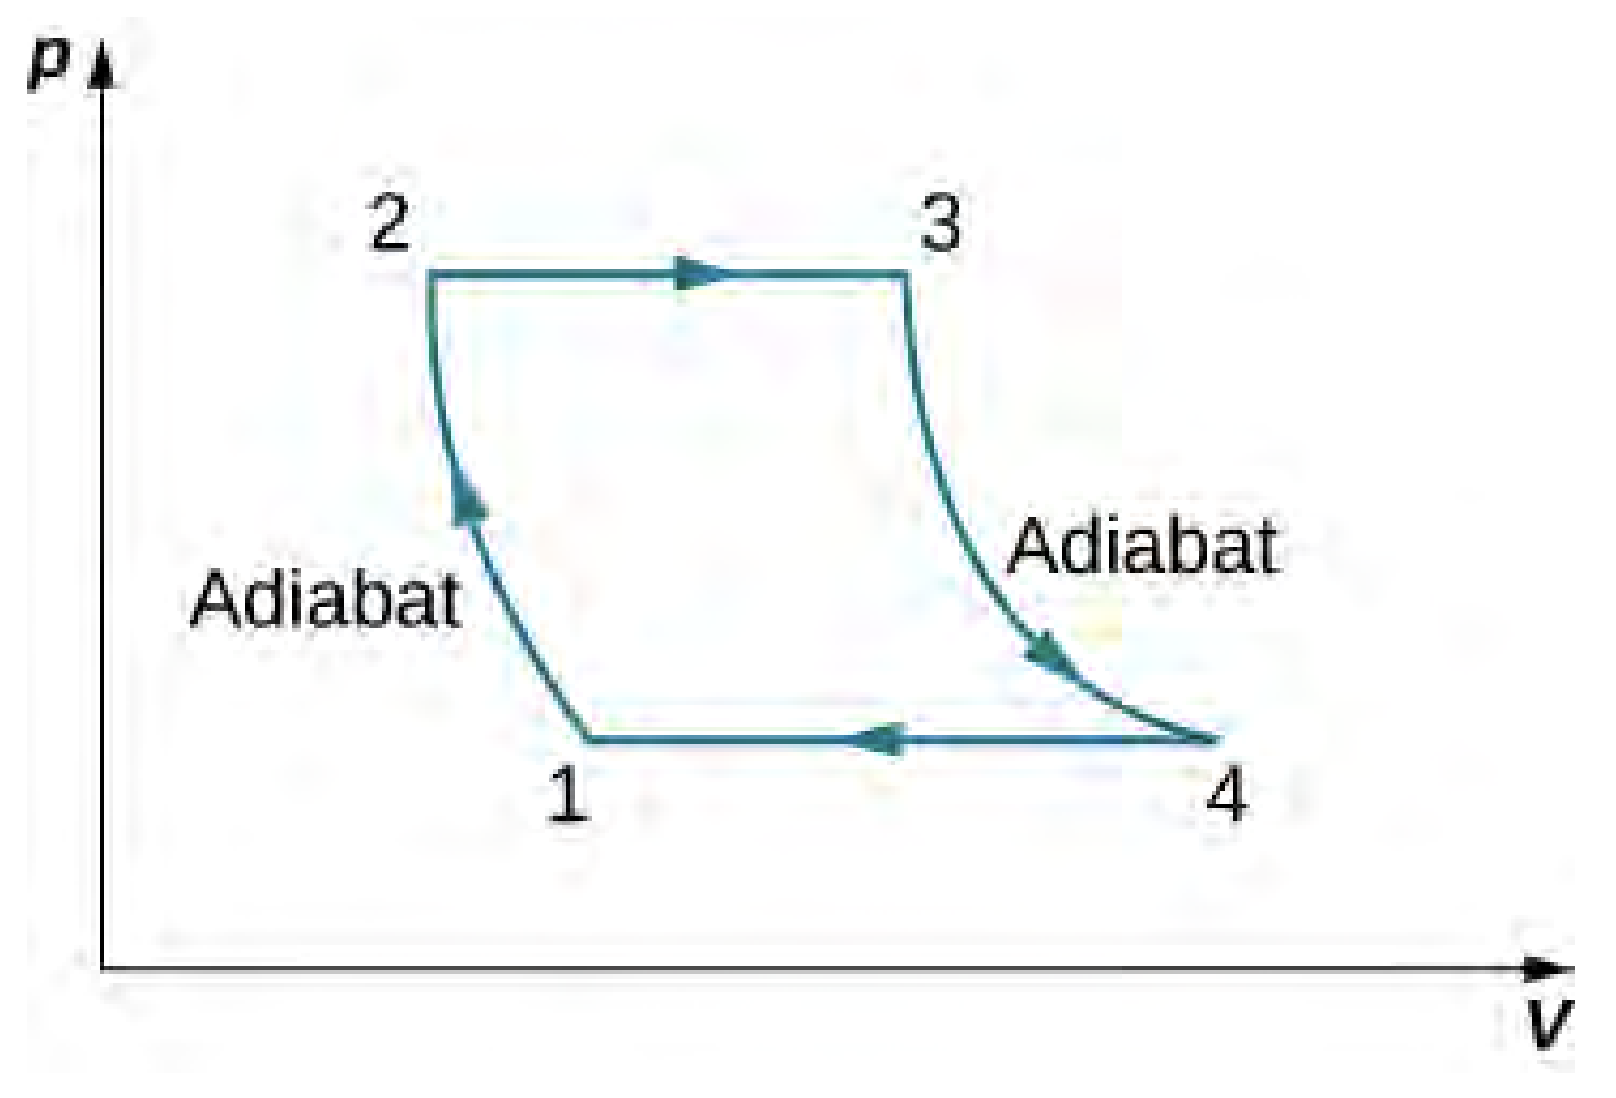
\includegraphics[scale=0.35]{4-90.png}
\end{document}
